\documentclass[11en, a4paper, oneside]{article}
\usepackage[utf8]{inputenc}   % <<<<< Linux
\usepackage[english]{babel} % <<<<< English
\usepackage{notoccite}
\usepackage[skip=0.5\baselineskip]{caption}
\hyphenation{GTKWave}
\usepackage{listings}
\usepackage[all]{nowidow}
\usepackage{tabularx}
\usepackage{amsmath}
\usepackage{float}

%blind text
\usepackage{lipsum}

\usepackage{graphicx}
\graphicspath{ {./} {../../figlib/} }
\def\FontLn{% 16 pt normal
  \usefont{T1}{phv}{m}{n}\fontsize{16pt}{16pt}\selectfont}
\def\FontLb{% 16 pt bold
  \usefont{T1}{phv}{b}{n}\fontsize{16pt}{16pt}\selectfont}
\def\FontMn{% 14 pt normal
  \usefont{T1}{phv}{m}{n}\fontsize{14pt}{14pt}\selectfont}
\def\FontMb{% 14 pt bold
  \usefont{T1}{phv}{b}{n}\fontsize{14pt}{14pt}\selectfont}
\def\FontSn{% 12 pt normal
  \usefont{T1}{phv}{m}{n}\fontsize{12pt}{12pt}\selectfont}

% Use Arial font as default
%
\renewcommand{\rmdefault}{phv}
\renewcommand{\sfdefault}{phv}
\usepackage{geometry}	
\geometry{verbose,tmargin=2.5cm,bmargin=2.5cm,lmargin=2.5cm,rmargin=2.5cm}

%\usepackage{setspace}
%\renewcommand{\baselinestretch}{1.5}

\usepackage[pdftex]{hyperref} % enhance documents that are to be
                              % output as HTML and PDF
\hypersetup{colorlinks,       % color text of links and anchors,
                              % eliminates borders around links
%            linkcolor=red,    % color for normal internal links
            linkcolor=black,  % color for normal internal links
            anchorcolor=black,% color for anchor text
%            citecolor=green,  % color for bibliographical citations
            citecolor=black,  % color for bibliographical citations
%            filecolor=magenta,% color for URLs which open local files
            filecolor=black,  % color for URLs which open local files
%            menucolor=red,    % color for Acrobat menu items
            menucolor=black,  % color for Acrobat menu items
%            pagecolor=red,    % color for links to other pages
            pagecolor=black,  % color for links to other pages
%            urlcolor=cyan,    % color for linked URLs
            urlcolor=black,   % color for linked URLs
	          bookmarks=true,         % create PDF bookmarks
	          bookmarksopen=false,    % don't expand bookmarks
	          bookmarksnumbered=true, % number bookmarks
	          pdftitle={report},
            pdfauthor={Andre C. Marta},
%            pdfsubject={Thesis Title},
%            pdfkeywords={Thesis Keywords},
            pdfstartview=FitV,
            pdfdisplaydoctitle=true}

\usepackage[numbers,sort&compress]{natbib} % <<<<< References in numbered list [1],[2],...
\usepackage{subcaption} 
\usepackage{mdframed}
\usepackage[utf8]{inputenc}
\usepackage{graphicx}
\usepackage{amsmath}
\usepackage{indentfirst}
\usepackage{fancyhdr}
\usepackage{hyperref}
\usepackage{subfiles}
\usepackage{wrapfig}
\usepackage{subcaption}
\usepackage[utf8]{inputenc}
%\usepackage[nottoc]{tocbibind}
\usepackage{lastpage}
\newcommand{\clap}{\makebox[0pt]}
\usepackage{titlesec}
\usepackage{amsfonts}
\usepackage{listings}
\usepackage{color} %red, green, blue, yellow, cyan, magenta, black, white
\definecolor{mygreen}{RGB}{28,172,0} % color values Red, Green, Blue
\definecolor{mylilas}{RGB}{170,55,241}
\newcommand{\overbar}[1]{\mkern 1.5mu\overline{\mkern-1.5mu#1\mkern-1.5mu}\mkern 1.5mu}
\titleformat{\paragraph}
{\normalfont\normalsize\bfseries}{\theparagraph}{1em}{}
\titlespacing*{\paragraph}
{0pt}{3.25ex plus 1ex minus .2ex}{1.5ex plus .2ex}
\geometry{margin=0.67in}

\usepackage{etoolbox}
\patchcmd{\thebibliography}{\section*{\refname}}{}{}{}

\graphicspath{ {./Imagens/} }

\hypersetup{colorlinks,citecolor=black,filecolor=black,linkcolor=black,urlcolor=black} 

\lstset{language=Matlab,%
    %basicstyle=\color{red},
    breaklines=true,%
    morekeywords={matlab2tikz},
    keywordstyle=\color{blue},%
    morekeywords=[2]{1}, keywordstyle=[2]{\color{black}},
    identifierstyle=\color{black},%
    stringstyle=\color{mylilas},
    commentstyle=\color{mygreen},%
    showstringspaces=false,%without this there will be a symbol in the places where there is a space
    numbers=left,%
    numberstyle={\tiny \color{black}},% size of the numbers
    numbersep=9pt, % this defines how far the numbers are from the text
    emph=[1]{for,end,break},emphstyle=[1]\color{red}, %some words to emphasise
    %emph=[2]{word1,word2}, emphstyle=[2]{style},    
}


\pagestyle{fancy}
\fancyhf{}
\rhead{Circuit Theory and Electronics Fundamentals}
\lhead{Group 21}
\cfoot{Página  \thepage \hspace{1pt} de \pageref{LastPage}}
\pagenumbering{roman}

\begin{document}


\begin{titlepage}
	\begin{center}
		\begin{figure}[htb!]
			\begin{center}
				\includegraphics[width=10cm]{tecnico.png}
			\end{center}
		\end{figure}
		
        \vspace{30pt}
        \begin{center}
        \Large{\center Integrated Masters in Aerospace Engineering, Técnico, University of Lisbon}\\
        \Large{\center Circuit Theory and Electronics Fundamentals}\\
        \end{center}
            
        \vspace{60pt}
        \Huge{\textbf{Laboratory Report 2}}
        
        \vspace{120pt}
        \begin{minipage}{0.4\textwidth}
		\begin{flushleft} \large
			\emph{\LARGE{\textbf{Grupo 21:}}}\par \vspace{10pt}
			95791, Francisco Carvalho \\ \vspace{20pt}
            95805, João Matias\\ \vspace{20pt}
            95846, Simão Gonçalves\\ \vspace{20pt}
		\end{flushleft}
	\end{minipage}
	~
	\begin{minipage}[b]{0.4\textwidth}
		\begin{flushright} \large
        	{}
		\end{flushright}
	\end{minipage}\\[2cm]
       \vspace{10pt}
        \large{April 2021}\\
	\end{center}
\end{titlepage}

\newpage
\renewcommand{\contentsname}{Índice}
\tableofcontents
\thispagestyle{empty}

\newpage
\pagenumbering{arabic}
\setcounter{page}{3}

\section{Introduction}

For the second experimental activity in the Circuit Theory and Electronics Fundamentals course, we were given a RC circuit to analyse.
This circuit is constituted by a sinusoidal voltage source $v_s$, dependent voltage $V_d$ and current $I_b$ sources, a capacitor $C$ and 7 resistors (fig. \ref{intro}).

The theoretical analysis (Section \ref{sec:analysis}) adresses, sequencially, the nodal analysis, then the calculus of $R_{eq}$. With these results, the natural response of the circuit, the forced response are computed, and then superimposed.

The simulation analysis (Section \ref{simuanal}) was made to validate the results obtained in section \ref{sec:analysis}, operating point, transient and then frequency analysis were made in Ngspice.
The conclusions of this study are outlined in the final section (\ref{resan}).

The voltage source varies in time as it follows:



\begin{equation}
v_s(t) = V_s u(-t) + sin(2\pi ft)u(t)
\end{equation}
where
\begin{equation}
u(t)=\begin{cases} 0, \quad t<0 \\ 1, \quad t \geq 0  \end{cases}
\end{equation}


To obtain the initial data, we ran a python script provided by our teacher, which generated the following data:\\

\begin{table}[h]
\centering
\begin{tabularx}{0.6\textwidth} {
  | >{\raggedright\arraybackslash}X
  | >{\raggedleft\arraybackslash}X | }
 \hline
R1 & 1.048998e+03 kOhm\\ \hline
R2 & 2.055568e+03 kOhm\\ \hline
R3 & 3.060188e+03 kOhm\\ \hline
R4 & 4.168980e+03 kOhm\\ \hline
R5 & 3.073950e+03 kOhm\\ \hline
R6 & 2.042810e+03 kOhm\\ \hline
R7 & 1.037563e+03 kOhm\\ \hline
Vs & 5.114229e+00 V\\ \hline
C & 1.011550e-06 uF\\ \hline
Kb & 7.338555e-03 mS\\ \hline
Kd & 8.258180e+03 kOhm\\ \hline

\end{tabularx}
\caption{Initial Data generated by the python script. The variables are expressed in V, mA, mS, kOhm, uF.}
\end{table}

\begin{figure}[ht] \centering
\includegraphics[width=0.7\linewidth]{Circuito1.pdf}
\caption{Solução natural $v_{6n}(t)$, $t\in[0,20]$ ms}
\label{fig:snat}
\end{figure}

\begin{figure}[ht] \centering
\includegraphics[width=0.7\linewidth]{Circuito2.pdf}
\caption{Solução natural $v_{6n}(t)$, $t\in[0,20]$ ms}
\label{fig:snat}
\end{figure}

\clearpage

\section{Theoretical Analysis}
\label{Teorica}
\subsection{Gain Stage Description}

Firstly, we will make a brief description of how the gain stage works. As previously stated, its objective is to amplify the voltage input. In order to do so we utilize the following components: NPN BJT (negative-positive-negative bipolar junction transistor), Resistors, Capacitors and voltage sources.

The $V_{cc}$ voltage source is added with the objective of ensuring the transistor is acting in the Forward Active Region. The condition for operating in such region is $V_{CE}>V_{BE}$.

Both the capacitors have important functions within the circuit. The $C_{in}$ capacitor (coupling capacitor) acts as a DC block, ensuring that the transistor is in the desired operating region. The second capacitor, $C_E$, is a bypass capacitor. Taking a look at the formulae for the capacitor impedance: $\frac{1}{jwc}$, we can understand what this means. For low frequencies, the capacitor impedance is really high, which makes all the current flow through the RE resistor. On the other hand, for high frequencies, the capacitor impedance is really low, making it act almost as a short circuit. Therefore, almost all current flows through it.

It is also relevant to look at the impedance seen by the input voltage source, as it needs to be a lot greater than the resistance associated with the generator. The formulae is the following:

\begin{equation}
    Z_{I1}= (R_1 || R2) || r_{\pi 1}
\end{equation}


Taking a look at the output impedance formulae (\ref{form1}), we can see that it is really high, in comparison to the load resistance of 8 Ohm. Therefore, by the voltage divider rule, it becomes obvious that we need to add another stage to lower the impedance seen by the load. (note that we are doing a high-frequency analysis, considering $R_E \simeq 0$)

\begin{equation}
\label{form1}
     Z_{O1}=r_o || R_C
\end{equation}

\subsection{Output Stage Description}

As said before, the main goal of the output stage is to lower the output impedance.


For this stage, we utilized resistors, a capacitor, a PNP BJT and a voltage source.
Similarly to what was described in the previous stage, the voltage source is used to ensure the transistor operates in the desired region (forward active region), satisfying the condition for PNP BJT: $V_{EC}>V_{EB}$. Furthermore, the capacitor $C_O$ also acts as a coupling transistor, blocking the DC and ensuring the transistor stays in the forward active region.


Again, it is also relevant to look at the impedance seen by the input voltage source (\ref{form2}), as it needs to be much lower than $Z_{O1}$, so that there is no loss between both stages (voltage divider formulae, equation X). 

\begin{equation}
\label{form2}
    Z_{I2}=\frac{(g_{m2}+g_{\pi2}+g_{o2}+g_{E2})}{g_{\pi2}(g_{\pi2}+g_{o2}+g_{E2})}
\end{equation}

\begin{equation}
    V_{in2} = \frac{Z_{I2}}{Z_{I2}+Z_{O1}} V_{O2}. 
\end{equation}


Taking a look at the output impedance formulae (\ref{form3}), we that the output stage achieves its purpose of diminishing the impedance seen by the load.

\begin{equation}
\label{form3}
     Z_{O2}=\frac{1}{(g_{m2}+g_{\pi2}+g_{o2}+g_{E2})}
\end{equation}




\subsection{Merit Figure and Values Determination}

The main goal of this lab was to design the best possible audio amplification circuit. The quality of our work is evaluated with the calculation of a merit figure, which takes into account the following parameters:
-the voltage gain between the voltage generator input, and the load output; 
-the lower cut-off frequency (and higher cut-off frequency), which corresponds to the minimum (and maximum) frequency value of the bandwidth, and represents the first (and last) frequency for which the signal is correctly amplified, which is desired to be as low (as high) as possible. Both these frequencies are calculated by determining when the output voltage is 3db less than the gain;
-the bandwidth of our amplified signal, which is the range of frequencies for which our input signal is correctly amplified (it's calculated by subtracting the higher cut-off frequency by the lower cut-off frequency);
-the cost of the circuit.

The formulae for the merit figure is the following:


With the objective to obtain the biggest possible merit figure, we ran an optimization using Simulink, a very useful toolbox of the Matlab program. With this, we obtained the following values for our resistors and capacity of the capacitors:

\begin{table}[H]
\centering
\begin{tabularx}{0.6\textwidth} {
  | >{\raggedright\arraybackslash}X
  | >{\raggedleft\arraybackslash}X | }
 \hline
VCE & 6.698985e+00 V\\ \hline
VBEON & 7.000000e-01 V \\ \hline
VEC & 7.503512e+00 V\\ \hline
VEBON & 7.000000e-01 V \\ \hline
IB1 & 5.816344e-06 A \\ \hline
IC1 & 1.039381e-03 A \\ \hline
IE1 & 1.045197e-03 A \\ \hline
IB2 & -3.285189e-05 A \\ \hline
IC2 & 7.467235e-03 A \\ \hline
IE2 & 7.500087e-03 A \\ \hline
Merit & 4.922026e+02 \\ \hline
HighCutOff frequency & 4.378919e+05 Hz\\ \hline
LowCutOff frequency & 1.262636e+01 Hz\\ \hline
Cost & 2.198944e+03 MU's\\ \hline
Bandwidth & 4.378793e+05 Hz\\ \hline
Max Gain & 3.111592e+01 V\\ \hline

\end{tabularx}
\caption{Optimization results and merit}
\end{table}

After discovering all the needed values, we can also plot the gain, input and output impedances of both the circuits.

\begin{table}[H]
\centering
\begin{tabularx}{0.6\textwidth} {
  | >{\raggedright\arraybackslash}X
  | >{\raggedleft\arraybackslash}X | }
 \hline
AV1dB & 3.158539e+01 dB\\ \hline
ZI1 & 2.419648e+03 Omega \\ \hline
ZO1 & 4.652785e+03 Omega \\ \hline

\end{tabularx}
\caption{Gain stage: gain in dB, input and output impedance}
\end{table}

\begin{table}[H]
\centering
\begin{tabularx}{0.6\textwidth} {
  | >{\raggedright\arraybackslash}X
  | >{\raggedleft\arraybackslash}X | }
 \hline
\input{ponto3_tab.tex}
\end{tabularx}
\caption{Output stage: gain in dB, input and output impedance}
\end{table}

\begin{table}[H]
\centering
\begin{tabularx}{0.6\textwidth} {
  | >{\raggedright\arraybackslash}X
  | >{\raggedleft\arraybackslash}X | }
 \hline
AVdB & 3.120876e+01 dB\\ \hline
ZO & 2.270796e+01 Omega\\ \hline

\end{tabularx}
\caption{Total circuit gain and output impedance}
\end{table}

And, finally, the frequency response $\frac{V_o(f)}{V_i(f)}$

\begin{figure}[H]\centering
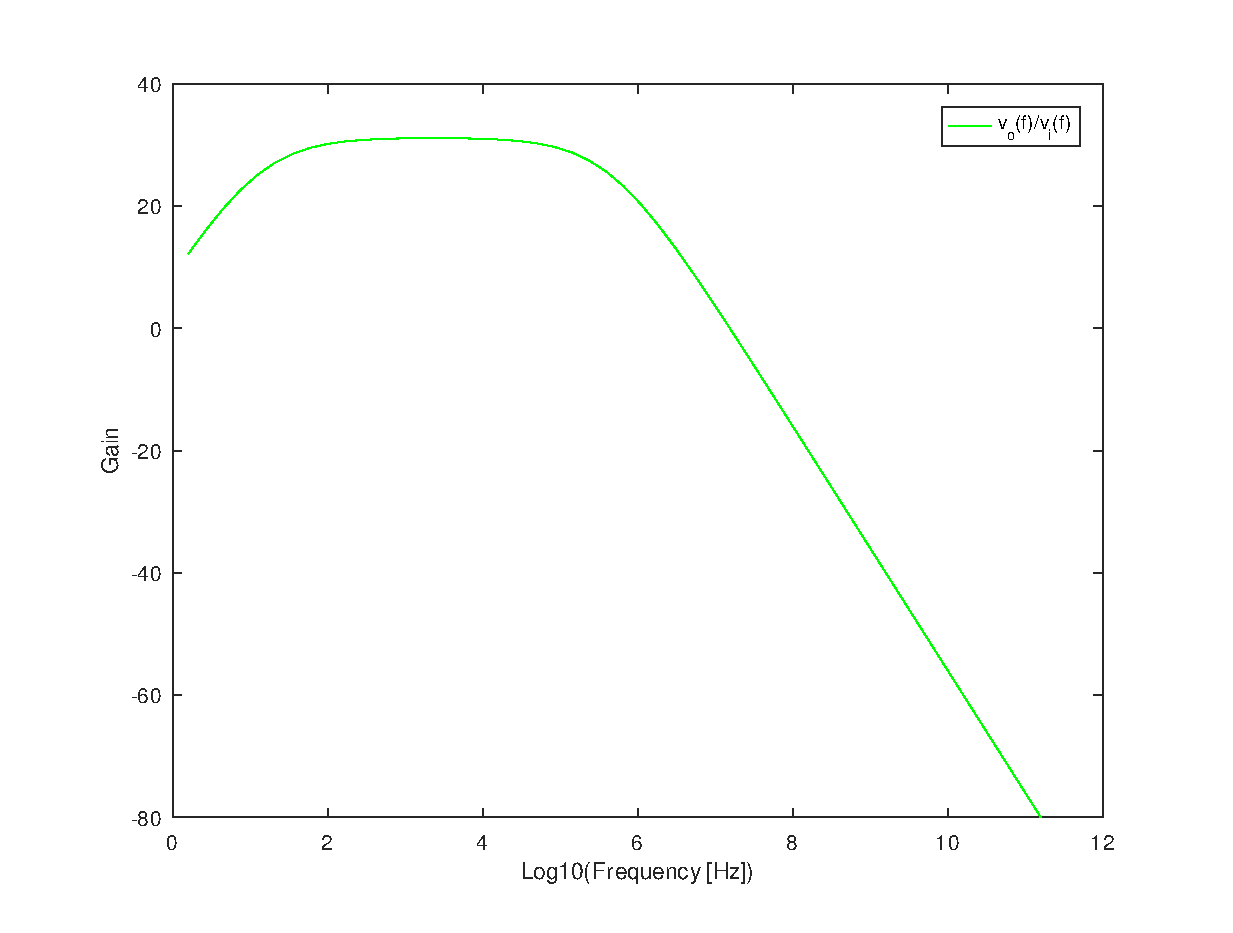
\includegraphics[width=0.7\linewidth]{grafico_octave.eps}
\caption{Octave Frequency response}
\label{fig:snat}
\end{figure}



\section{Simulation Analysis}
\label{simuanal}

In order to understand the values obtained in our simulation, it is important to note a couple of things:
\begin{itemize}
    \item Node 4 is considered to be ground, therefore, its' voltage is not shown in the table of results, but is, obviously, 0V.
    \item To compute the voltage drop through the dependent voltage source ($V_d$), we needed to obtain
the current value through resistor R6. However, Ngspice doesn’t allow us to input Resistor $R_6$ current in the computation. Hence, in order to solve this problem, we introduced a voltage source
with no voltage drop in series with the $R_6$ resistor. This way, we managed to obtain the current
through it, and therefore we were able to compute the dependent voltage source $V_d$.
\end{itemize}

\subsection{Circuit Analysis for $t \leq 0 $}

For $t < 0$, the voltage source (Va) is producing a constant voltage source of value Vs. Therefore, the capacitor behaves as an open circuit. After running the Ngspice script, we obtained the following results:

\begin{table}[h]
\centering
\begin{tabularx}{0.6\textwidth} {
  | >{\raggedright\arraybackslash}X
  | >{\raggedleft\arraybackslash}X | }
 \hline
@gb[i] & -2.39986e-04\\ \hline
@r1[i] & -2.29300e-04\\ \hline
@r2[i] & -2.39986e-04\\ \hline
@r3[i] & -1.06863e-05\\ \hline
@r4[i] & 1.176882e-03\\ \hline
@r5[i] & -2.39986e-04\\ \hline
@r6[i] & 9.475819e-04\\ \hline
@r7[i] & 9.475819e-04\\ \hline
v(1) & 5.114229e+00\\ \hline
v(2) & 4.873694e+00\\ \hline
v(3) & 4.380386e+00\\ \hline
v(5) & 4.906396e+00\\ \hline
v(6) & 5.644101e+00\\ \hline
v(7) & -1.93573e+00\\ \hline
v(8) & -2.91891e+00\\ \hline
v(9) & -1.93573e+00\\ \hline

\end{tabularx}
\caption{Nodal Voltage Simulation Results. Variables expressed in V or A}
\end{table}

\begin{table}[h]
\centering
\begin{tabularx}{0.6\textwidth} {
  | >{\raggedright\arraybackslash}X
  | >{\raggedleft\arraybackslash}X | }
 \hline
V1 & 5.114229e+00 V\\ \hline
V2 & 4.873694e+00 V\\ \hline
V3 & 4.380386e+00 V\\ \hline
V4 & 0.000000e+00 V\\ \hline
V5 & 4.906396e+00 V\\ \hline
V6 & 5.644102e+00 V\\ \hline
V7 & -1.935730e+00 V\\ \hline
V8 & -2.918905e+00 V\\ \hline

\end{tabularx}
\caption{Theoretical Nodal Voltages expressed in V}
\end{table}

\begin{table}[h]
\centering
\begin{tabularx}{0.6\textwidth} {
  | >{\raggedright\arraybackslash}X
  | >{\raggedleft\arraybackslash}X | }
 \hline
I1 & -2.293000e-04 A\\ \hline
I2 & -2.399863e-04 A\\ \hline
I3 & -1.068631e-05 A\\ \hline
I4 & 1.176882e-03 A\\ \hline
I5 & -2.399863e-04 A\\ \hline
I6 & 9.475818e-04 A\\ \hline
I7 & 9.475818e-04 A\\ \hline
Is & -2.293000e-04 A\\ \hline
Ic & 0.000000e+00 A\\ \hline

\end{tabularx}
\caption{Theoretical Nodal Voltages expressed in A}
\end{table}

\subsection{$R_{eq}$ Calculus, and Circuit Analysis for $t=0$}

In the second simulation, the open circuit branch of the capacitor was replaced with a voltage source, with voltage $V_x=V_6-V_8$. This step was needed to calculate the equivalent Thévenin resistance, which can be obtained through the following expression:
\begin{equation}
     R_{eq}=\frac{V_6-V_8}{I_x}
\end{equation}


with $I_x$ being the current through the voltage source previously defined $V_x$.

\begin{table}[h]
\centering
\begin{tabularx}{0.6\textwidth} {
  | >{\raggedright\arraybackslash}X
  | >{\raggedleft\arraybackslash}X | }
 \hline
\input{Q2_tab.tex}
\end{tabularx}
\caption{Nodal Voltage Simulation results. Variables expressed in V}
\end{table}

\begin{table}[h]
\centering
\begin{tabularx}{0.6\textwidth} {
  | >{\raggedright\arraybackslash}X
  | >{\raggedleft\arraybackslash}X | }
 \hline
V1 & 0.000000e+00 V\\ \hline
V2 & -1.114084e-17 V\\ \hline
V3 & 0.000000e+00 V\\ \hline
V4 & 0.000000e+00 V\\ \hline
V5 & -5.941780e-17 V\\ \hline
V6 & 8.563007e+00 V\\ \hline
V7 & 0.000000e+00 V\\ \hline
V8 & 0.000000e+00 V\\ \hline
Ix & -2.785669e-03 A\\ \hline
Req & 3.073950e+03 Ohm\\ \hline
tau & 3.109455e-03 \\ \hline

\end{tabularx}
\caption{Theoretical results expressed in V, A and Ohm}
\end{table}

\newpage
\subsection{Circuit Analysis for $t \geq 0 $ (Natural Solution)}

For the third simulation, we performed a transient analysis of the given circuit, which is similar to the one done in the previous section. The main difference is the introduction of the capacitor instead of the voltage source between nodes 6 and 8, and the fact that the voltage source is turned off. With this, we run the Ngspice script to obtain the natural solution of the circuit.

\begin{figure}[h!]\centering
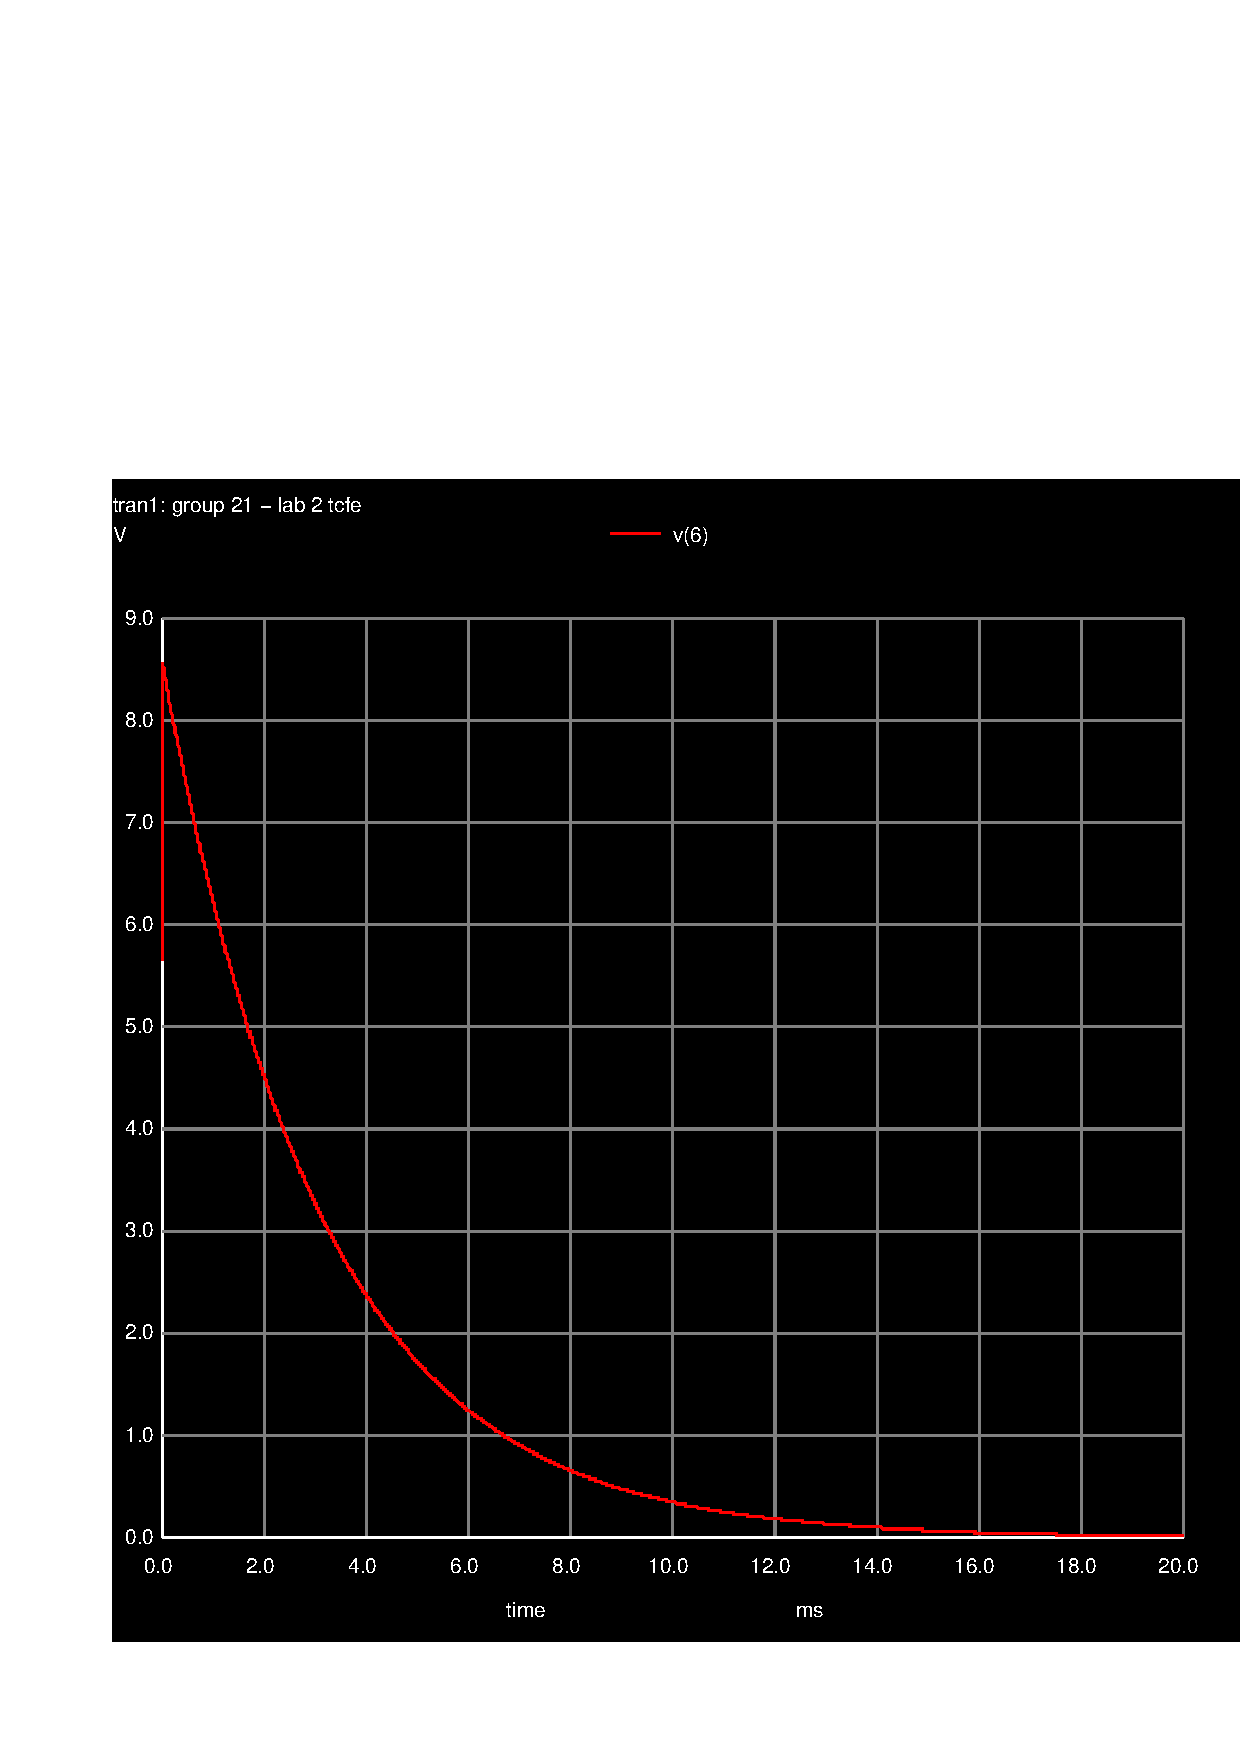
\includegraphics[width=0.5\linewidth]{question_3.pdf}
\caption{Natural Solution (Ngspice)}
\label{fig:snat}
\end{figure}

\begin{figure}[h!] \centering
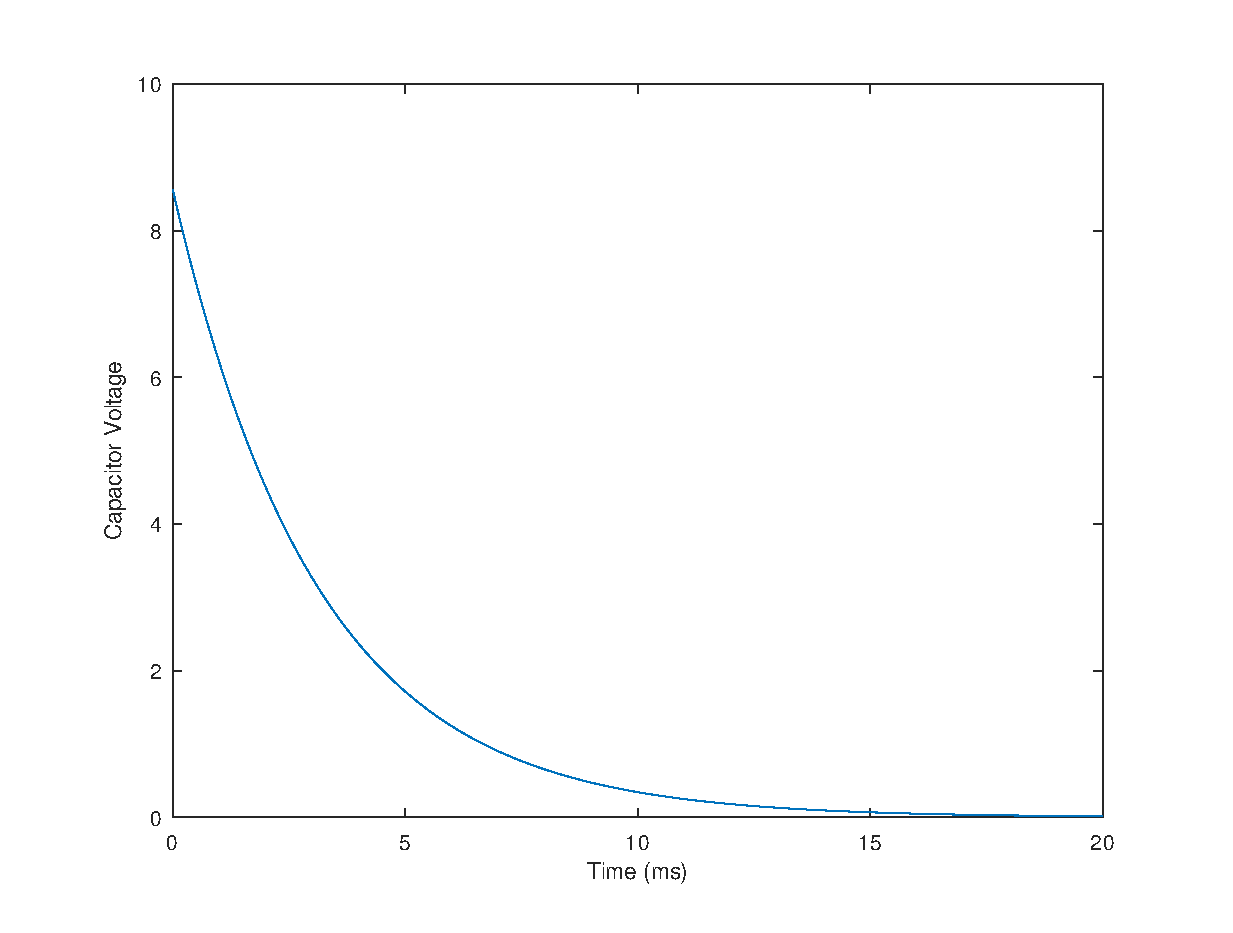
\includegraphics[width=0.5\linewidth]{naturalsolution.eps}
\caption{Natural Solution (Octave)}
\label{fig:snat}
\end{figure}


We can conclude that the capacitor is discharging over time, as expected, concluding that the theoretical analysis and the simulation, match.

\newpage
\subsection{Circuit Analysis for $t \geq 0 $ (Natural and Forced Solution)}

In this section we also performed a transient analysis, making a few changes to the circuit, in order to obtain a plot of the natural and forced solution. Therefore, we took in consideration the sinusoidal variation of the voltage source over time, plotting that in our computation.

\begin{figure}[h!] \centering
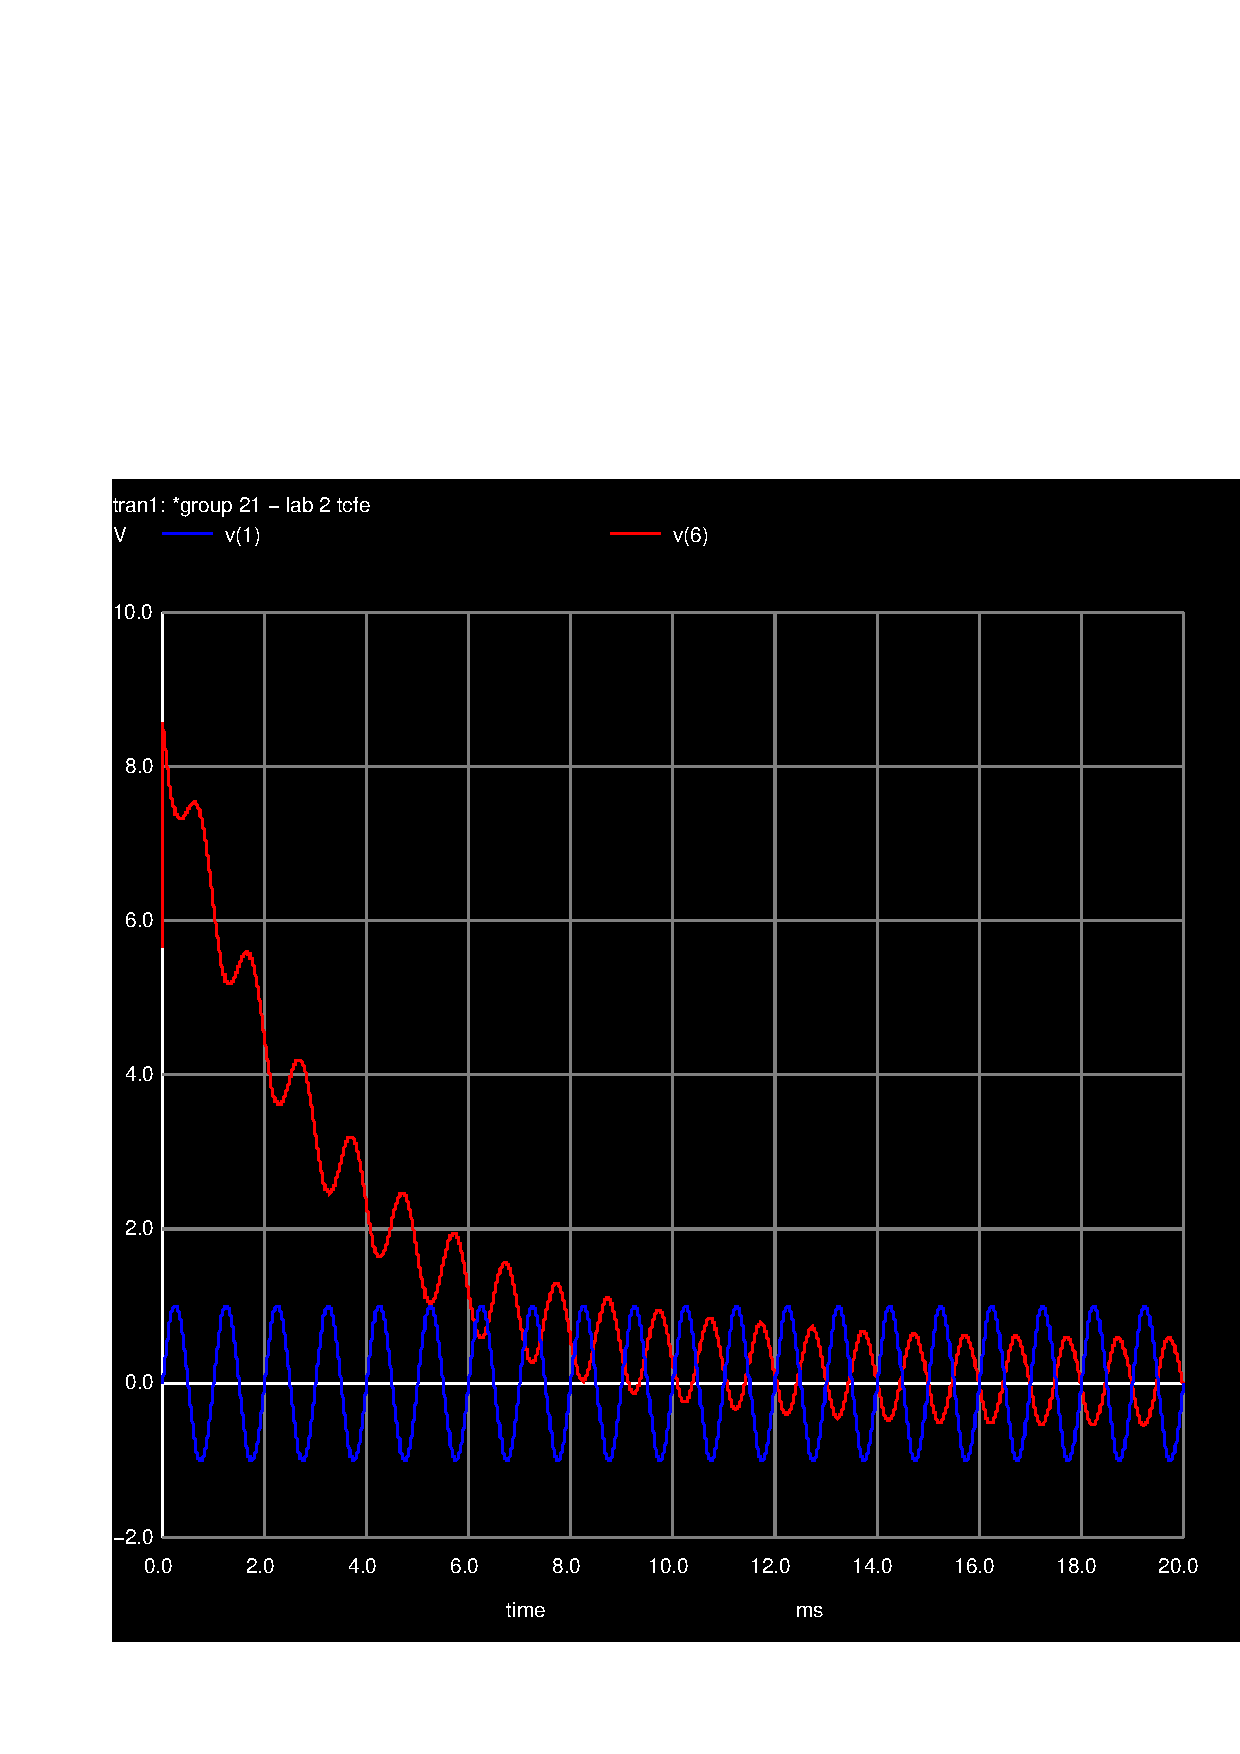
\includegraphics[width=0.5\linewidth]{question_4.pdf}
\caption{Final Solution (NGSpice)}
\label{fig:snat}
\end{figure}

\begin{figure}[h!] \centering
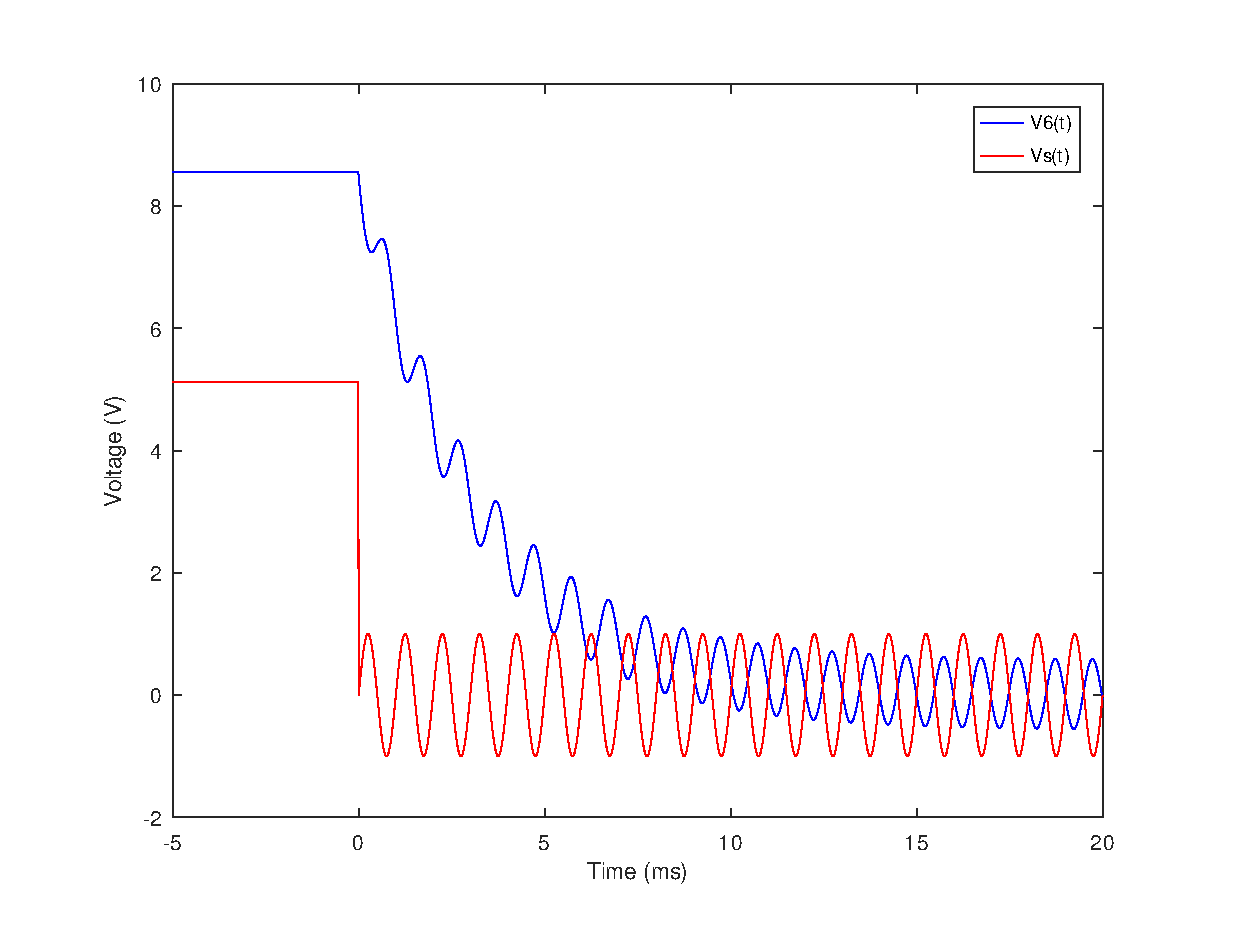
\includegraphics[width=0.6\linewidth]{forced_and_natural_solution.eps}
\caption{Final Solution (Octave)}
\label{fig:snat}
\end{figure}

As we can see from the pictures above, both Octave and Ngspice results match perfectly. W can conclude that the voltage in the capacitor diminishes until it has a phase difference of $\pi$, in comparison to the voltage source, as expected in the theoretical analysis.
\newpage
\subsection{Frequency Responses}

For this section, we conducted and Alternating Current (AC) Analysis. With this, we were able to study the frequency response of the circuit. It is important to note that there is no frequency variation, which means we are performing a steady-state analysis. After examination of the graphics below, it is clear that the results from Octave match the ones of Ngspice clear, where any minor difference may be explained by approximation errors.

\subsubsection{Frequency Responses - Amplitude}

\begin{figure}[h!]
\centering
\begin{subfigure}{.5\textwidth}
  \centering
  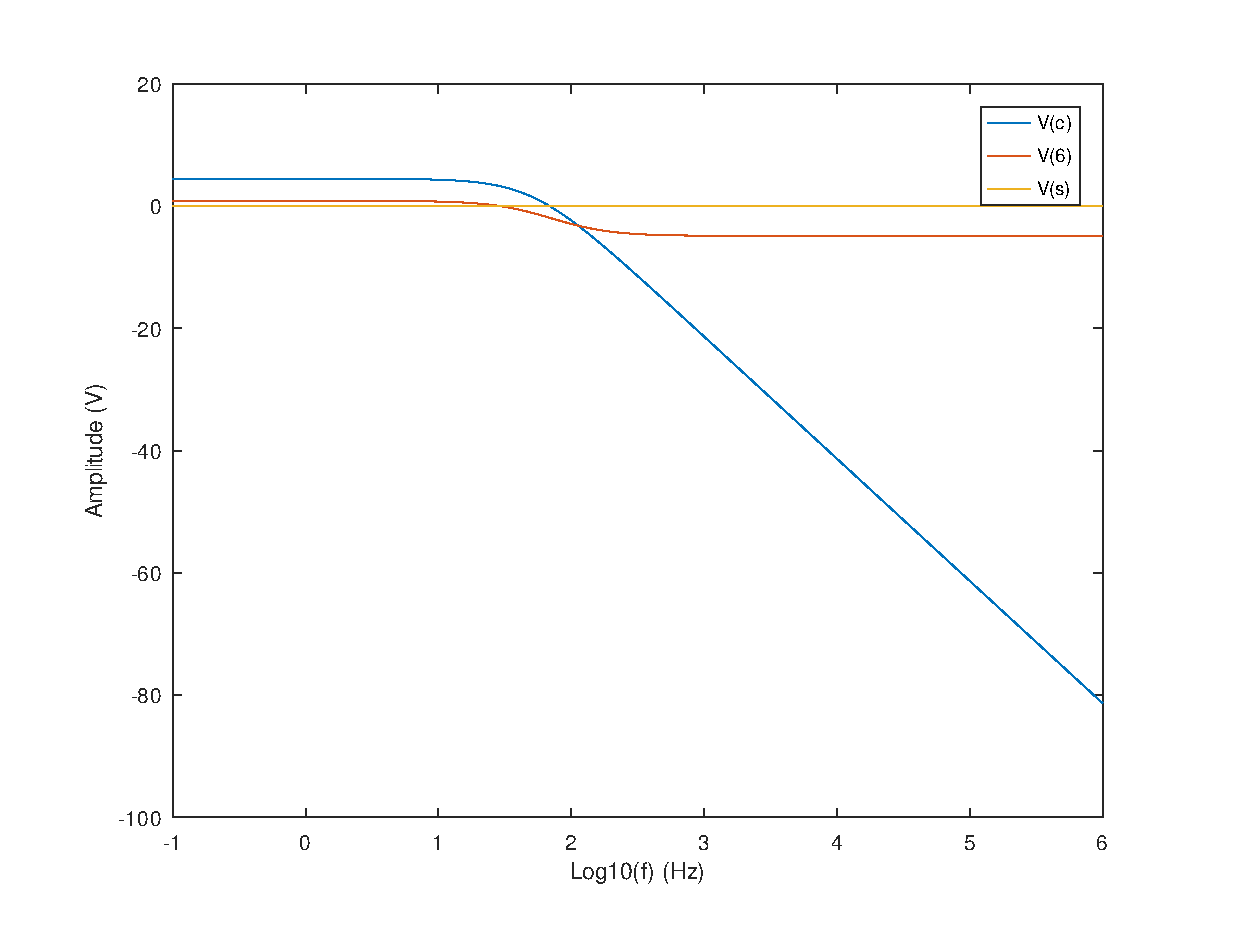
\includegraphics[width=.9\linewidth]{amplitude.eps}
  \captionof{figure}{Amplitude (Octave)}
  \label{fig:test1}
\end{subfigure}%
\begin{subfigure}{.5\textwidth}
  \centering
  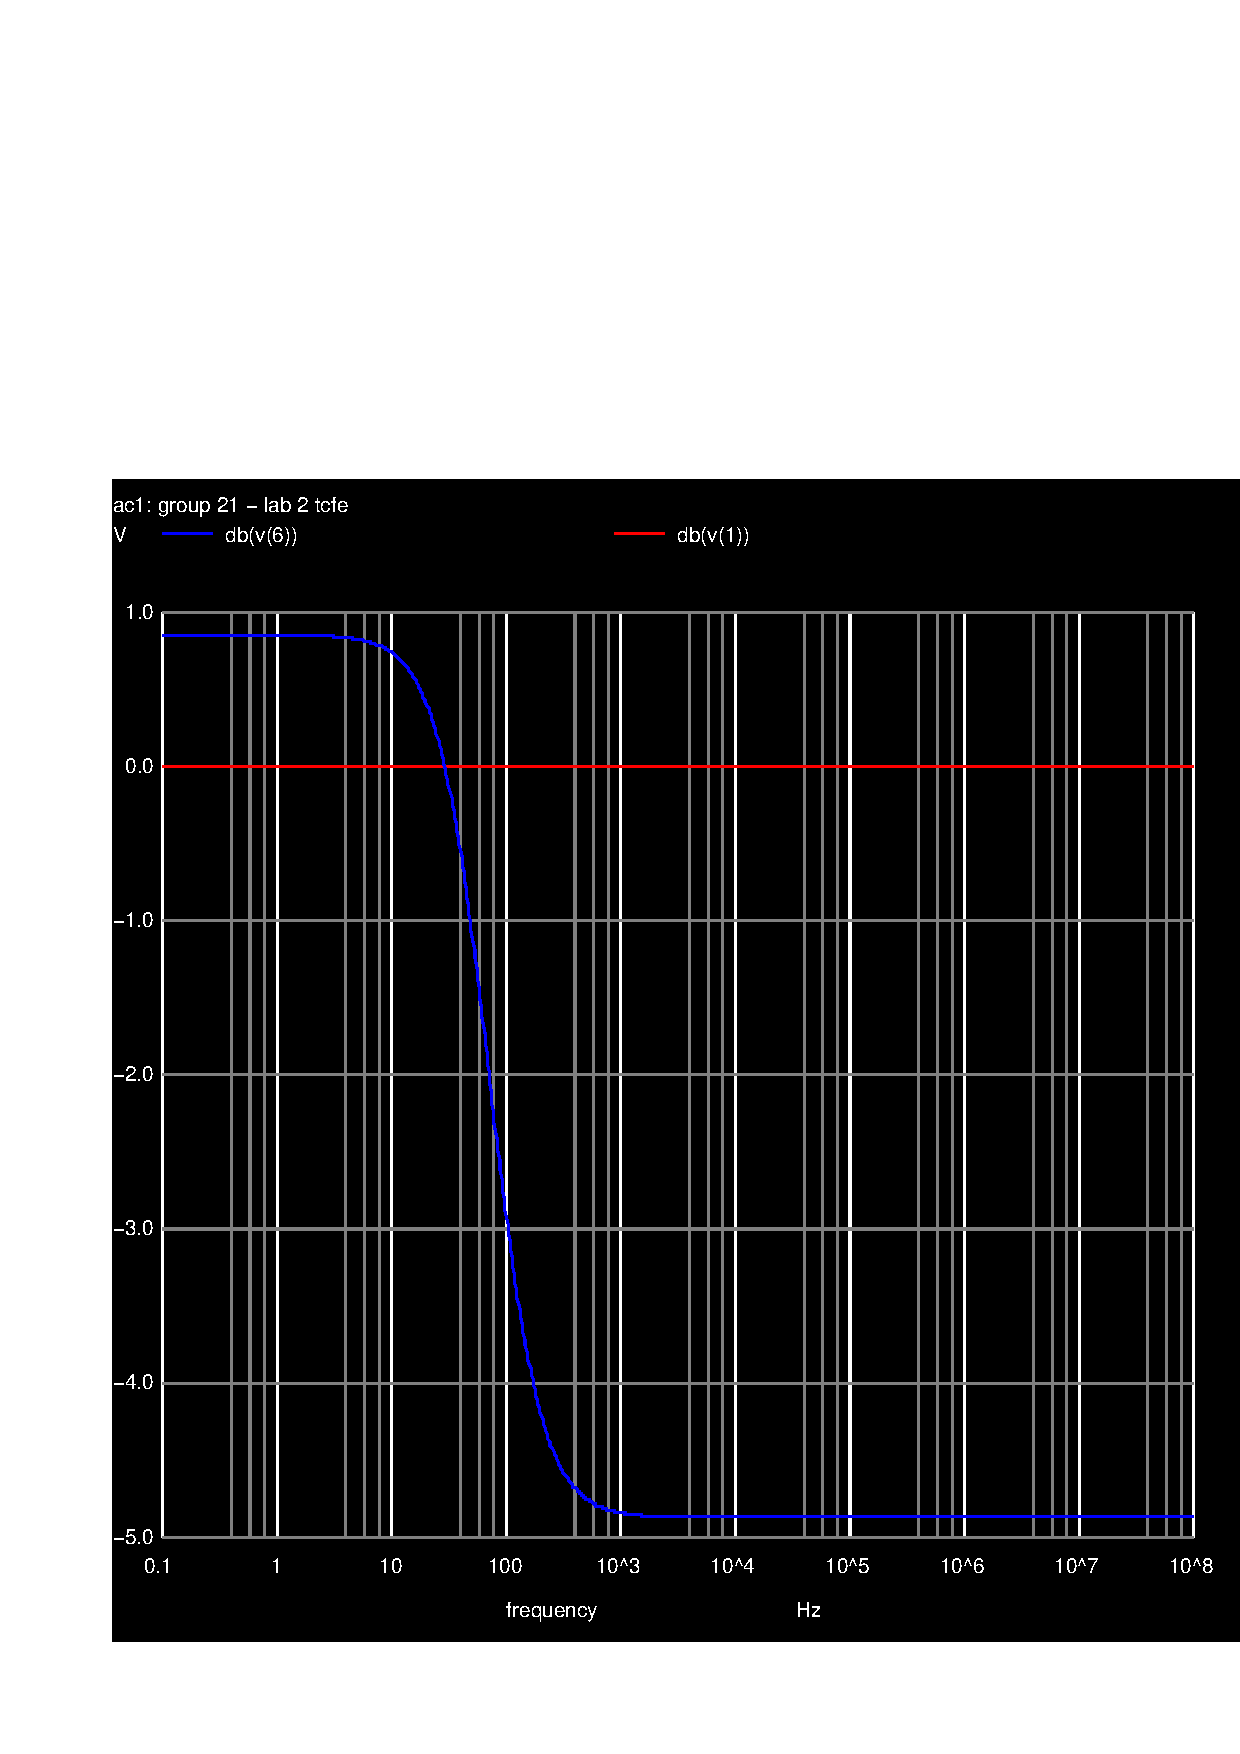
\includegraphics[width=.9\linewidth]{question5_db.pdf}
  \captionof{figure}{Amplitude (Ngspice}
  \label{fig:test2}
\end{subfigure}
\end{figure}

\newpage
\subsubsection{Frequency Responses - Phase}

\begin{figure}[h!]
\centering
\begin{subfigure}{.5\textwidth}
  \centering
  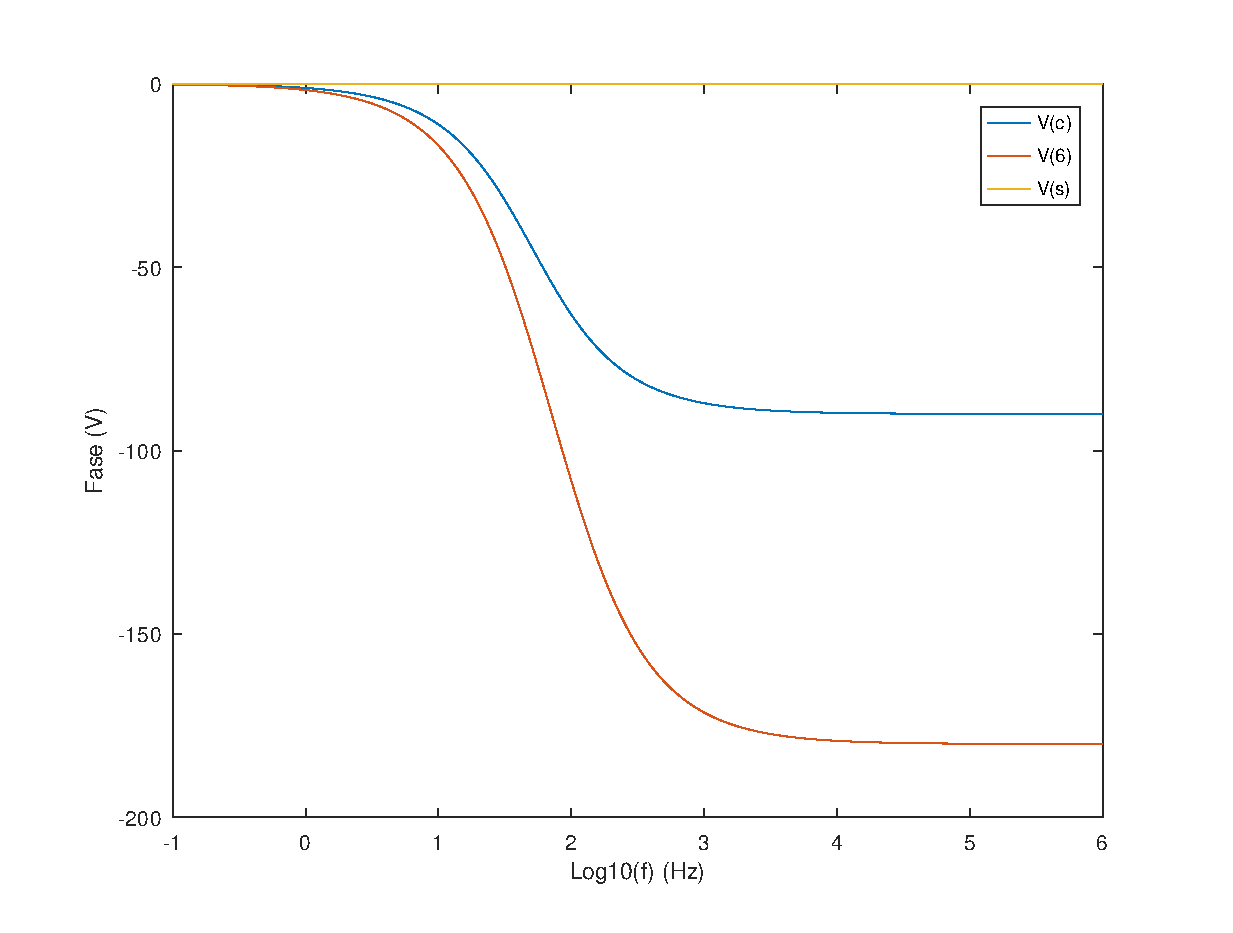
\includegraphics[width=.9\linewidth]{phase.eps}
  \captionof{figure}{Phase (Octave)}
  \label{fig:test1}
\end{subfigure}%
\begin{subfigure}{.5\textwidth}
  \centering
  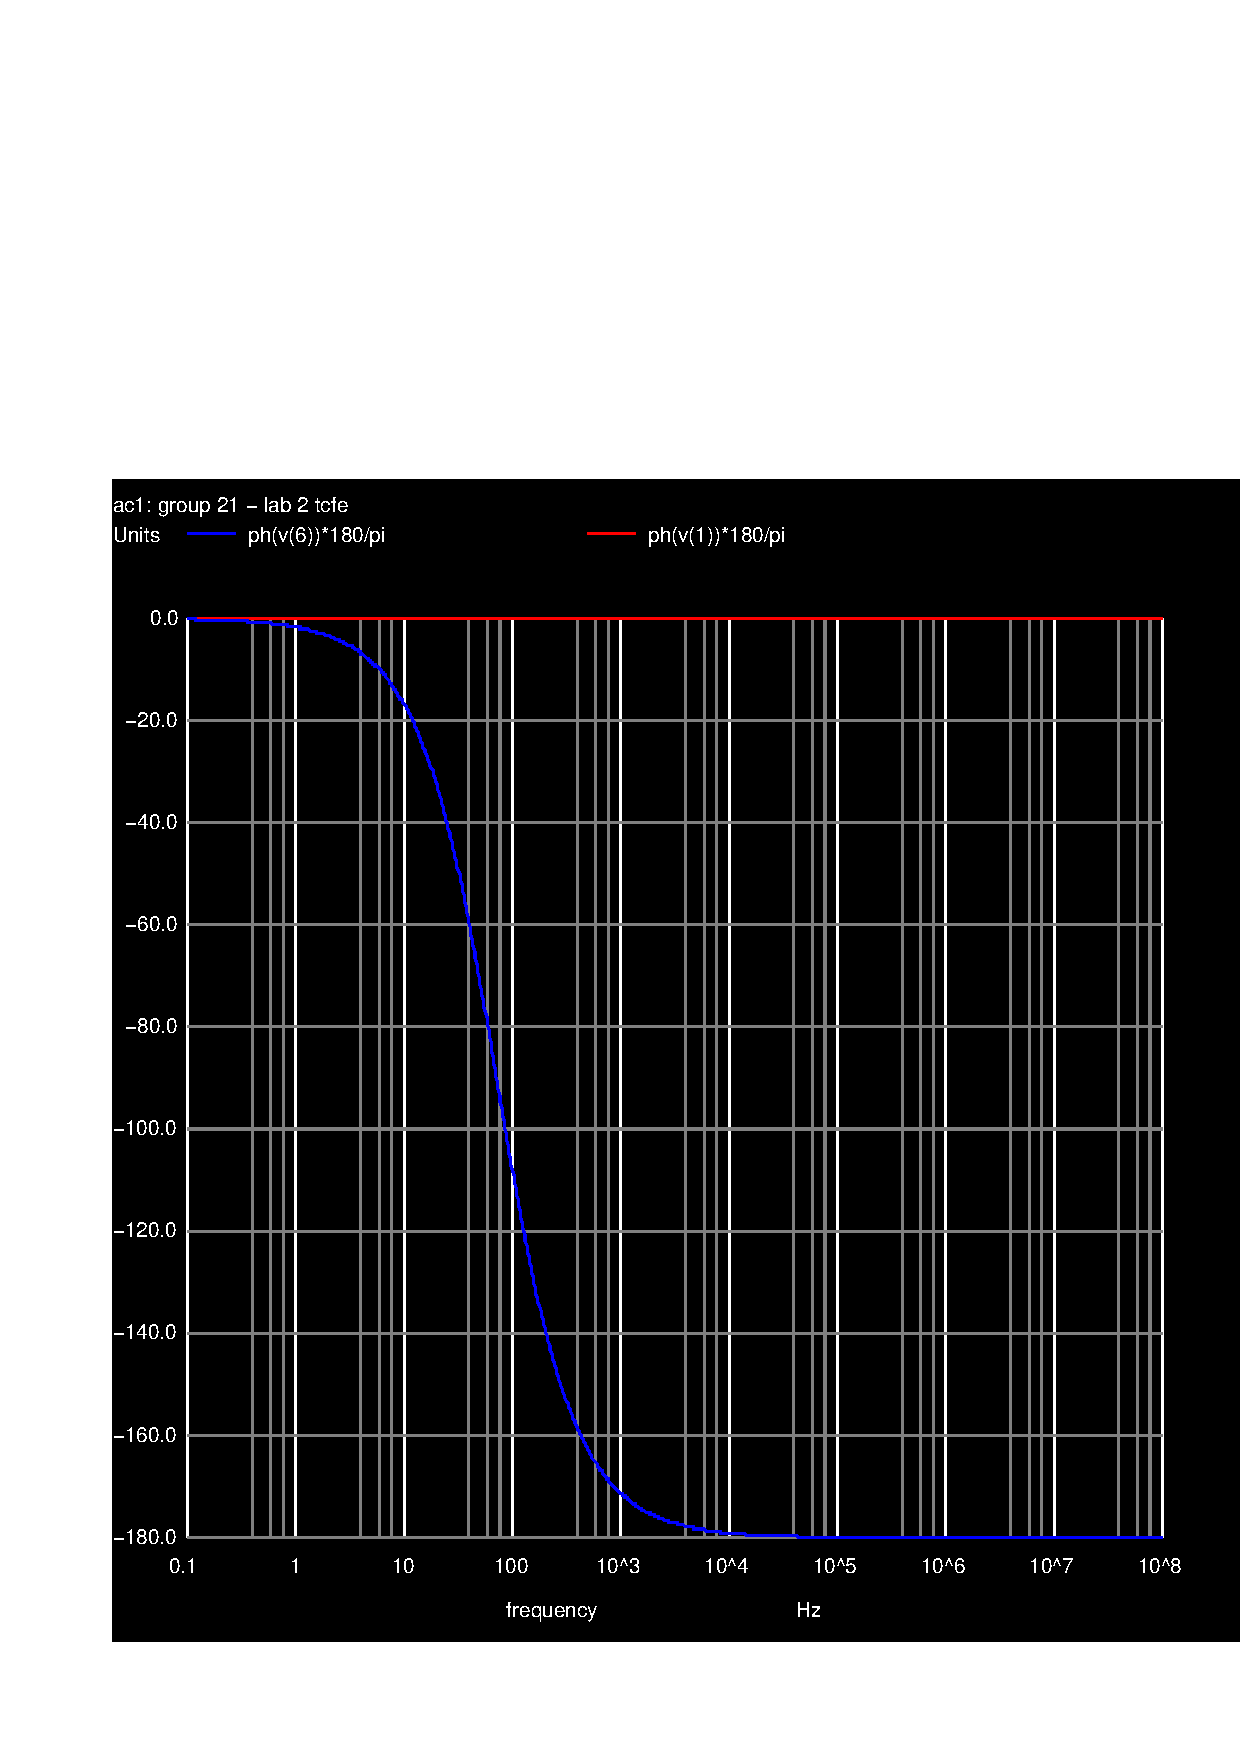
\includegraphics[width=.9\linewidth]{question5_ph.pdf}
  \captionof{figure}{Phase (Ngspice)}
  \label{fig:test2}
\end{subfigure}
\end{figure}

\section{Conclusion}
\label{resan}
All analyses have been performed both theoretically using the Octave maths tool and by circuit simulation using the Ngspice tool.
As we can see the both theorical and simulation results match for every single component of the circuit. Even though we could have expected a bigger error margin due to the number of circuit components and the number of steps to get to final awnser, that was not the case. Hence, the circuit analysis proposed in the introduction was achieved.








\end{document}

